%Hallo Andrin
% main.tex -- Paper zum Thema <parallelisierung>
%
% (c) 2020 Autor, OST Ostschweizer Fachhochschule
%
% !TEX root = ../../buch.tex
% !TEX encoding = UTF-8
%
\chapter{Thema\label{chapter:parallelisierung}}
\kopflinks{Thema}
\begin{refsection}
\chapterauthor{Andrin Kälin, Andrin Rütsche}

Ein paar Hinweise für die korrekte Formatierung des Textes
\begin{itemize}
\item
Absätze werden gebildet, indem man eine Leerzeile einfügt.
Die Verwendung von \verb+\\+ ist nur in Tabellen und Arrays gestattet.
\item
Die explizite Platzierung von Bildern ist nicht erlaubt, entsprechende
Optionen werden gelöscht. 
Verwenden Sie Labels und Verweise, um auf Bilder hinzuweisen.
\item
Beginnen Sie jeden Satz auf einer neuen Zeile. 
Damit ermöglichen Sie dem Versionsverwaltungssysteme, Änderungen
in verschiedenen Sätzen von verschiedenen Autoren ohne Konflikt 
anzuwenden.
\item 
Bilden Sie auch für Formeln kurze Zeilen, einerseits der besseren
Übersicht wegen, aber auch um GIT die Arbeit zu erleichtern.
\end{itemize}

%
% teil1.tex -- Beispiel-File für das Paper
%
% (c) 2020 Prof Dr Andreas Müller, Hochschule Rapperswil
%
% !TEX root = ../../buch.tex
% !TEX encoding = UTF-8
%
\section{Lokalität
\label{parallelisierung:sec:Lokalitaet}}
\kopfrechts{Lokalität}
Lokalität beschreibt den Umstand, dass ein physikalischer oder mathematischer Vorgang nur von seiner unmittelbaren Umgebung beeinflusst wird. 
Dieses Konzept ist zentral für das Verständnis vieler physikalischer Prozesse und bildet zugleich die Grundlage für numerische Verfahren, mit denen wir Feldgleichungen berechnen können. 
Ohne die Annahme der Lokalität wäre es nicht möglich, komplexe Systeme in Teilprobleme zu zerlegen und effizient auf Rechnerarchitekturen umzusetzen.

\subsection{Lokalität im physikalischen Sinn
	\label{parallelisierung:sub:LokalitaetPhysik}}
Auf einfache Weise lässt sich Lokalität am Beispiel der Wärmeleitung veranschaulichen. 
Die Temperatur an einem bestimmten Ort hängt nicht unmittelbar von allen Punkten im Material ab, sondern nur von den direkt benachbarten Zellen. 
Der Wärmestrom ergibt sich lokal aus den Temperaturdifferenzen zwischen einem Punkt und seinen Nachbarn.
Eine heiße Stelle in einem Metallblock beeinflusst also nicht direkt eine weit entfernte Stelle, sondern nur die benachbarten Bereiche. 
Diese Nachbarstellen wiederum beeinflussen die nächsten, und so breitet sich Wärme schrittweise aus. 
Es gibt Beispiele von Fernwirkung in der Physik wie zum Beispiel das newton`sche Gravitationsgesetz oder Coulombs Gesetz für elektrische Ladung.
Diese sind für viele Anwendungen sehr nützlich, es sind aber nur vereinfachte Gesetze.
In der modernen Physik können jedoch alle physikalischen Prozesse durch Felder mit streng lokalen Wechselwirkungen erklärt werden.
Es gibt ausserhalb der Quantenmechanik keine echte Fernwirkung in der Physik.

\subsection{Lokalität im mathematischen Sinn
\label{parallelisierung:sub:LokalitaetMathematik}}
In der Mathematik tritt Lokalität vor allem bei Differentialoperatoren auf. 
Eine Ableitung an einer Stelle beschreibt das Verhalten einer Funktion in einer sehr kleinen Umgebung dieses Punktes. 
In der numerischen Mathematik, wo kontinuierliche Operatoren durch diskrete Approximationen ersetzt werden, wird dieses Prinzip besonders deutlich. 
So wird etwa eine erste Ableitung durch Differenzen zwischen benachbarten Gitterpunkten dargestellt, und eine zweite Ableitung durch Kombination dieser Differenzen. 
Damit greift die Berechnung stets nur auf Werte aus der unmittelbaren Nachbarschaft zu. 
Diese Eigenschaft macht Differentialoperatoren lokal und ermöglicht die Umsetzung auf Gittern.

\subsection{Lokalität und PDEs
\label{parallelisierung:sub:LokalitaetPDE}}
Für partielle Differentialgleichungen (PDEs) ist die Lokalität von zentraler Bedeutung. 
Die Veränderung einer Größe in Raum und Zeit hängt immer nur von den lokalen Gradienten oder Krümmungen ab. 
Würde ein Operator auf das gesamte Feld wirken, könnte man die Gleichung nicht sinnvoll numerisch lösen. 
Zudem ist Lokalität entscheidend für die Parallelisierung, denn nur da jedes Teilgebiet seine Lösung ausschließlich aus lokalen Informationen berechnen kann, lassen sich deren Berechnungen auf mehrere Prozessoren verteilen. 
Lediglich an den Grenzen der Teilgebiete muss kommuniziert werden, um den Austausch der Randzellen sicherzustellen. 
Somit bildet Lokalität nicht nur die theoretische Grundlage für PDEs, sondern auch die praktische Voraussetzung für deren effiziente Berechnung auf modernen Rechnerarchitekturen.


%
% einleitung.tex -- Beispiel-File für die Einleitung
%
% (c) 2020 Prof Dr Andreas Müller, Hochschule Rapperswil
%
% !TEX root = ../../buch.tex
% !TEX encoding = UTF-8
%
\section{Numerische Methoden}
\kopfrechts{Numerische Methoden}

Bisher wurden Feldgleichungen und deren Lösungen aus einer theoretischen und abstrakten Perspektive betrachtet.
Dies ist grundlegend für das Verständnis der zugrundeliegenden Konzepte.

Um den praktischen Nutzen dieser mächtigen Theorie jedoch voll auszuschöpfen, ist ein Übergang von dieser idealisierten, kontinuierlichen und grenzenlosen Sichtweise hin zu einer realitätsnahen, diskreten und physikalisch eingeschränkten Betrachtung erforderlich.
Konkret bedeutet dies, dass wir die Feldgleichungen diskretisieren müssen.

Ein prominentes Beispiel dafür ist das numerische Wettermodell des ECMWF (European Centre for Medium-Range Weather Forecasts), das auf Grundlage eines breiten Spektrums aktueller und vergangener Wetterdaten versucht, möglichst präzise Vorhersagen für die kommenden zehn Tage zu treffen.

Als wichtigste und somit einflussreichste Parameter dieses Modells gelten der Luftdruck, die Lufttemperatur, die Windgeschwindigkeit bzw. -richtung, die Luftfeuchtigkeit sowie diverse Niederschlagsparameter \cite{ecmwf2023}.
Diese Messwerte liegen jedoch nur mit begrenzter zeitlicher und räumlicher Auflösung vor.

Sie bestimmen somit die Feinheit des zugrundeliegenden Datenrasters --- ein Umstand, der sich später als entscheidend erweisen wird.

\subsection{Diskretisierung statt Interpolation}

Angesichts der Tatsache, dass die Messwerte nur in diskreter Form vorliegen, stellt sich die Frage, warum man nicht versucht, diese durch geeignete Interpolation wieder in ein kontinuierliches Datenset zu überführen, um dann die bekannten kontinuierlichen Gleichungen analytisch auszuwerten.
Diese Fragestellung allein könnte den Umfang dieses gesamten Papers einnehmen.
Daher sollen im Folgenden nur einige ausgewählte, nicht abschließende Aspekte diskutiert werden.

Ein erster wesentlicher Punkt ist, dass Interpolation ein rein mathematisches Verfahren darstellt, das keinerlei physikalische Gesetzmäßigkeiten berücksichtigt.
In der Praxis führt dies dazu, dass verrauschte und durch das Abtasten bereits verfälschte Messwerte durch Interpolation weiter verfälscht werden können.

Eine mögliche Lösung wäre, die Interpolation um ein physikalisches Modell zu erweitern, sprich ein Kalman Filter, welches die Lücken auf möglichst plausible Weise schließt.
Dabei würde jedoch ein weiteres physikalisches Modell entstehen, das letztlich nur dazu dient, Daten für das eigentliche Modell zu liefern --- was den methodischen Aufwand verdoppelt, ohne zwingend zusätzliche Erkenntnisse zu bringen.

Ein weiterer zentraler Vorteil numerischer Verfahren liegt in ihrer Fähigkeit, auch Gleichungen zu lösen, die keine geschlossene analytische Lösung besitzen.
Dies ist insbesondere in der Strömungsmechanik von Bedeutung.
Ein Beispiel dafür ist die Navier-Stokes-Gleichung, welche die Bewegung von Flüssigkeiten und Gasen beschreibt.
Für den allgemeinen dreidimensionalen Fall ist bis heute keine Lösung in geschlossener Form bekannt.

Numerische Verfahren ermöglichen jedoch näherungsweise Lösungen mit vernachlässigbar kleinen Fehlern, sofern geeignete Diskretisierung und Randbedingungen gegeben sind.
Allen klassischen numerischen Methoden zur Lösung partieller Differentialgleichungen ist gemeinsam, dass sie das kontinuierliche, analytische Problem in ein algebraisches Gleichungssystem mit endlich vielen Unbekannten überführen.
Dieses lässt sich anschließend mit numerischen Verfahren der linearen Algebra effizient auf dem Computer lösen.

\subsection{Überblick über numerische Methoden zur Lösung von Feldgleichungen}

Zur numerischen Lösung partieller Differentialgleichungen existieren verschiedene etablierte Methoden, die je nach Anwendungsgebiet unterschiedliche Vor- und Nachteile aufweisen.
Drei der wichtigsten Verfahren werden im Folgenden kurz vorgestellt.

\subsubsection{Finite-Differenzen-Methode (FDM)}
\label{parallelisierung:section:fdm}

Die Finite-Differenzen-Methode ersetzt Ableitungen durch Differenzenquotienten auf einem diskreten Gitter.
Dadurch wird die ursprüngliche Differentialgleichung in ein algebraisches Gleichungssystem überführt, das die gesuchte Lösung an diskreten Gitterpunkten beschreibt.
FDM ist insbesondere für einfache Geometrien und regelmäßige Gitter gut geeignet und vergleichsweise leicht zu implementieren.
Sie wird häufig bei Wärmeleitungsproblemen, Diffusionsprozessen und einfachen Wellengleichungen verwendet.

\subsubsection{Finite-Elemente-Methode (FEM)}

Die Finite-Elemente-Methode basiert auf der schwachen Formulierung der Gleichung und verwendet eine Zerlegung des Lösungsgebiets in sogenannte Elemente (z.B. Dreiecke oder Tetraeder).
Innerhalb dieser Elemente wird die Lösung durch geeignete Basisfunktionen approximiert.
FEM ist besonders leistungsfähig für komplexe Geometrien, Materialinhomogenitäten und Randwertprobleme in der Elektrotechnik und Strömungsmechanik.

\subsubsection{Finite-Volumen-Methode (FVM)}

Die Finite-Volumen-Methode basiert auf der integralen Form der Erhaltungssätze (z.B. Massen-, Impuls- oder Energieerhaltung) und ist besonders geeignet für konservative Systeme, also Systeme, bei denen physikalische Erhaltungsgrößen wie Masse oder Energie nicht erzeugt oder vernichtet, sondern nur transportiert oder umgewandelt werden.
Die Methode berechnet Flüsse über die Ränder sogenannter Kontrollvolumina.
Sie ist weit verbreitet in der Computational Fluid Dynamics (CFD), insbesondere bei der Simulation von Strömungen, Gasdynamik und Transportprozessen.

\subsubsection{Wahl der Methode}

Für das im Folgenden betrachtete Beispiel --- die eindimensionale Wärmeleitungsgleichung --- ist die Finite-Differenzen-Methode besonders geeignet.
Die Geometrie ist einfach, und das Verfahren erlaubt eine direkte, transparente Umsetzung der zugrundeliegenden physikalischen Zusammenhänge in eine diskrete Form.
Daher wird im nächsten Abschnitt die FDM im Detail erläutert und anhand eines konkreten Beispiels demonstriert.

\subsection{Beispiel FDM}

Als Ausgangslage wird die allgemeine Wärmeleitungsgleichung
\begin{equation}
	\frac{\partial T}{\partial t}
	=
	\alpha \Delta T.
	\label{parallelisierung:eq:Wärmeleitung_alg}
\end{equation}
betrachtet.
Im folgenden wird im 2D-Raum gearbeitet, also resultiert
\begin{equation}
	\frac{\partial T}{\partial t}
	=
	\alpha \biggl(
	\frac{\partial^2 T}{\partial x^2}
	+
	\frac{\partial^2 T}{\partial y^2}
	\biggr).
	\label{parallelisierung:eq:Wärmeleitung_2D}
\end{equation}


\subsubsection{Diskretisierung der Variablen}

Als erstes müssen die Variablen diskretisiert werden. Dies tun wir indem wir ein Gitter über den gesamten Bereich (zeitlich, sowie räumlich) legen, also
Im Raum:
\begin{equation}
	x_i
	=
	i \cdot \Delta x,
\end{equation}
\begin{equation}
	y_j
	=
	j \cdot \Delta y,
\end{equation}
und in der Zeit:
\begin{equation}
	t_n
	=
	n \cdot \Delta t.
\end{equation}

Somit wird unsere resultierende, diskrete Temperaturfunktion die Form
\begin{equation}
	T^n_{i,j}
	=
	T(x_i,y_j,t_n)
\end{equation}
haben.


\subsubsection{Diskretisierung der Zeit}

Die partielle Ableitung der Temperaturfunktion \( T \) nach der Zeit wird durch eine explizite Vorwärtsdifferenz approximiert:

\begin{equation}
	\label{parallelisierung:eq:discrete_time_derivative}
	\left. \frac{\partial T}{\partial t}\right|{(i,j,n)}
	\approx
	\frac{T_{i,j}^{n+1} - T_{i,j}^n}{\Delta t}.
\end{equation}
Dies entspricht der zeitlichen Änderungsrate von \( T \) am diskreten Gitterpunkt \( (x_i, y_j, t_n) \).

\subsubsection{Diskretisierung des Raums}
Auch hier beginen wir mit der einmaligen Anwendungen des Differentialquotienten (vorwärts), um die erste Ableitung, zunächst in $x$-Richtung zu approximieren:

\begin{equation}
	\left. \frac{\partial T}{\partial x} \right|{(i,j,n)}
	\approx \frac{T_{i+1,j}^n - T_{i,j}^n}{\Delta x}.
\end{equation}
Zusätzlich bestimmen wir den Differentialquotienten an einem vorangehenden Gitterpunkt
\begin{equation}
	\left. \frac{\partial T}{\partial x} \right|{(i-1,j,n)}
	\approx \frac{T_{i,j}^n - T_{i-1,j}^n}{\Delta x},
\end{equation}
um mittels einer letzen Anwendung des Differentialquotienten die Änderung dieser beiden Änderungen, also genau das was die zweite Ableitung beschreibt, diskret zu bestimmen
\begin{equation}
	\frac{\partial^2 T}{\partial x^2} \approx
	\frac{ \biggl( \frac{T_{i+1,j}^n - T_{i,j}^n}{\Delta x} \biggr) - \biggl( \frac{T_{i,j}^n - T_{i-1,j}^n}{\Delta x} \biggr) }{\Delta x}.
\end{equation}
Schlussendlich vereinfacht sich dies zu 
\begin{equation}
	\label{parallelisierung:eq:discrete_x_derivative}
	\left. \frac{\partial^2 T}{\partial x^2} \right|{(i,j,n)} \approx \frac{T_{i+1,j}^n - 2T_{i,j}^n + T_{i-1,j}^n}{(\Delta x)^2}.
\end{equation}
Für die y-Richtung folgt analog
\begin{equation}
	\label{parallelisierung:eq:discrete_y_derivative}
	\left. \frac{\partial^2 T}{\partial y^2} \right|{(i,j,n)} \approx \frac{T_{i,j+1}^n - 2T_{i,j}^n + T_{i,j-1}^n}{(\Delta y)^2}.
\end{equation}


Nun setzen wir die in den Formeln \eqref{parallelisierung:eq:discrete_time_derivative},  \eqref{parallelisierung:eq:discrete_x_derivative} und \eqref{parallelisierung:eq:discrete_y_derivative} gefundenen Gleichungen in die ursprüngliche zweidimensionale Wärmeleitungsgleichung Formel \eqref{parallelisierung:eq:Wärmeleitung_2D} ein.
Somit erhalten wir 

\begin{equation}
	\label{parallelisierung:eq:update_formula_unsorted}
	\frac{T_{i,j}^{n+1} - T_{i,j}^n}{\Delta t}
	=
	\alpha \biggl(
	\frac{T_{i+1,j}^n - 2 T_{i,j}^n + T_{i-1,j}^n}{(\Delta x)^2}
	+
	\frac{T_{i,j+1}^n - 2 T_{i,j}^n + T_{i,j-1}^n}{(\Delta y)^2}
	\biggr),
\end{equation}
womit die Diskretisierung der Wärmeleitungsgleichung mittels der Finite-Differenzen-Methode gezeigt ist.

\subsubsection{Explizite Updateformel}
\label{parallelisierung:sec:update_formel}


Aufgrund der Lokalität und Kausalität der Feldgleichungen ist die Temperatur eines Gitterpunkts \( (x_i, y_j)\) zu einem bestimmten Zeitpunkt in der Zukunft \( (t_{n+1})\) sprich \(T_{i,j}^{n+1}\) nur von dem  vorangegangenen Zustand eben dieses Gitterpunkts und desen direkten Nachbbaren abhängig.
Dies ist  in der nach \(T_{i,j}^{n+1}\) umgestellten Formel (\ref{parallelisierung:eq:update_formula_unsorted}) ersichtlich:
\begin{equation}
	\label{parallelisierung:eq:update_formula_sorted}
	T_{i,j}^{n+1}
	=
	T_{i,j}^n
	+
	\alpha \, \Delta t \biggl(
	\frac{T_{i+1,j}^n - 2 T_{i,j}^n + T_{i-1,j}^n}{(\Delta x)^2}
	+
	\frac{T_{i,j+1}^n - 2 T_{i,j}^n + T_{i,j-1}^n}{(\Delta y)^2}
	\biggr)
\end{equation}

Aus Übersichtsgründen fassen wir alle Konstanten (\(\alpha, \Delta t, \Delta x, \Delta y) \) zu einer neuen Konstanten zusammen.
Als praktische vereinfachung dazu legen wir fest, dass wir mit einem quadratischen Raumgitter arbeiten. Somit setzen wir  \(\Delta l = \Delta x = \Delta y\) und
\begin{equation}
	\label{parallelisierung:eq:lambda}
	\lambda 
	:= 
	\frac{\alpha \Delta t}{(\Delta l)^2}.
\end{equation}

Nun sind wir in der Lage, Formel \eqref{parallelisierung:eq:update_formula_sorted} kompakt und übersichtlich zu schreiben:

\begin{equation}
	\label{parallelisierung:eq:update_formel}
	T_{i,j}^{n+1}
	=
	T_{i,j}^n +
	\lambda \left(
	T_{i+1,j}^n + T_{i-1,j}^n + T_{i,j+1}^n + T_{i,j-1}^n - 4 T_{i,j}^n
	\right).
\end{equation}
Diese Formel wird als explizite Updateformel bezeichent, da sie iterativ auf Grundlage von gemesenen Daten oder zuvor berechneten Datenpunkten den nächsten Zeitschritt auswertet.

Es ist nun klar ersichtlich, dass die Temperatur an einem Punkt (\(x_i, y_j\)) zu einem gegebenen Zeitpunkt \(t_{n+1}\)  von der Temperatur an diesem Punkt zum Zeitpunkt \(t_n\) und der Wärmeflussbilanz zu den vier direkten Nachbarquadraten abhängig ist.

\subsubsection{Stabilitätskriterien}

Die in Gleichung~\eqref{parallelisierung:eq:lambda} eingeführte dimensionslose Konstante \(\lambda\) entscheidet, 
ob eine explizite FDM-Simulation stabil bleibt.  
Tabelle~\ref{parallelisierung:tab:stabilitaet_fdm} fasst die Stabilitätsbedingungen für Probleme verschiedener 
Dimensionen zusammen, wie sie aus einer Fourier-Analyse des Verstärkungsverhaltens einzelner Fehlerkomponenten 
resultieren.  
Aus Gründen der Lesbarkeit wird die vollständige Herleitung dieser Bedingungen an dieser Stelle nicht wiedergegeben; 
eine historische Einführung findet sich bereits bei Fourier \cite{Fourier1822}, während die systematische 
von-Neumann-Stabilitätsanalyse in \cite{VonNeumann1950} beschrieben ist.

\label{parallelisierung:sec:stabilitaetskriterien}

\begin{table}
	\centering
	\caption{Stabilitätsbedingungen der expliziten Finite-Differenzen-Methode}
	\label{parallelisierung:tab:stabilitaet_fdm}
	\begin{tabular}{|c|c|}
		\hline
		\textbf{Dimension} & \textbf{Stabilitätsbedingung} \\
		\hline
		1 & 
		\( \displaystyle \lambda = \frac{\alpha \, \Delta t}{(\Delta x)^2} \leq \frac{1}{2} \) \\
		\hline
		2 & 
		\( \displaystyle \lambda_x + \lambda_y =
		\frac{\alpha \, \Delta t}{(\Delta x)^2} +
		\frac{\alpha \, \Delta t}{(\Delta y)^2} \leq \frac{1}{2} \) \\
		\hline
		3 & 
		\( \displaystyle \lambda_x + \lambda_y + \lambda_z =
		\frac{\alpha \, \Delta t}{(\Delta x)^2} +
		\frac{\alpha \, \Delta t}{(\Delta y)^2} +
		\frac{\alpha \, \Delta t}{(\Delta z)^2} \leq \frac{1}{2} \) \\
		\hline
	\end{tabular}
\end{table}



Für den zweidimensionalen Fall gilt:
\begin{equation}
	\lambda_x + \lambda_y =
	\frac{\alpha \, \Delta t}{(\Delta x)^2} +
	\frac{\alpha \, \Delta t}{(\Delta y)^2} \leq \frac{1}{2}.
\end{equation}
Mit \(\Delta l = \Delta x = \Delta y\) folgt \(\lambda = \lambda_x = \lambda_y\), sodass sich die Formel zu
\begin{equation}
	\label{parallelisierung:eq:stabForExp}
	2\lambda = 2 \frac{\alpha \, \Delta t}{(\Delta l)^2} \leq \frac{1}{2}
	\quad \Rightarrow \quad
	\lambda = \frac{\alpha \, \Delta t}{(\Delta l)^2} \leq \frac{1}{4}
\end{equation}
ergibt.

\subsubsection{Physikalische Intuition}  
Man kann sich die Wärmeausbreitung wie das Füllen mehrerer miteinander verbundener Wasserbehälter vorstellen.  
Ist der Zeitabstand \(\Delta t\) zwischen den „Kontrollpunkten“ zu groß, können sich die Pegel zwischen den Behältern stark über- oder unterschwingen, anstatt sich gleichmäßig auszugleichen.  
Eine Erhöhung der thermischen Diffusivität \(\alpha\) wirkt ähnlich wie eine Verringerung der Viskosität einer Flüssigkeit: der Ausgleich erfolgt schneller, sodass kleinere Zeitintervalle notwendig werden.  
Auch eine Verringerung von \(\Delta x\) (feinere räumliche Auflösung) erfordert kleinere Zeitschritte, da die Temperaturunterschiede über kürzere Distanzen schneller wirken.
Im folgenden soll anhand von drei Experimenten die stabilität der Simulation, basierend auf der Updateformel  \eqref{parallelisierung:eq:update_formel}, genauer untersucht werden.

\subsubsection{Stabilitätsexperiment}

Zur Demonstration der Stabilitätsbedingung wird folgendes Szenario betrachtet:
Eine \(9 \times 9 \, \mathrm{cm}\) große Stahlplatte (ohne dritte Dimension) befindet sich in einer Umgebung mit konstanter Temperatur von \(0\,^{\circ}\mathrm{C}\).  
Die linke und rechte Kante werden konstant auf \(100\,^{\circ}\mathrm{C}\) gehalten.  
Das Material besitzt die Eigenschaften:
\begin{center}
	\begin{tabular}{llll}
		Wärmeleitfähigkeit & \(\kappa\) & 50 &
		\(\mathrm{W/(m \cdot K)}\) \\
		Dichte & \(\rho\)   &  7850 & \(\mathrm{kg/m^3}\) \\
		spezifische Wärmekapazität & \(c\) &  470 & \(\mathrm{J/(kg \cdot K)}\)
	\end{tabular}
\end{center}
Somit ergibt sich die thermische Diffusität zu


\[
\alpha =
\frac{\kappa}{\rho c}
=
\frac{50}{7850 \cdot 470}
= 1.355 \cdot 10^{-5}.
\]

\paragraph{Fall 1: Stabile Simulation}  
Mit \(100\) Messpunkten in einem \(10\times 10\)-Raster beträgt der Abstand \(\Delta l = 0.01\,\mathrm{m}\).  
Für \(\Delta t = 1\,\mathrm{s}\) ergibt sich
\[
\lambda =
\alpha \cdot \frac{\Delta t}{(\Delta l)^2}
=
10^{-5} \cdot \frac{1}{0.01^2}
\approx 0.135 < \frac14.
\]
Die Simulation konvergiert auf der Basis von \eqref{parallelisierung:eq:update_formel} nach 234 Iterationen zum stabilen Endzustand (Abbildung~\ref{parallelisierung:fig:simulation-10x10-0-135}).

\begin{figure}[htbp]
	\centering
	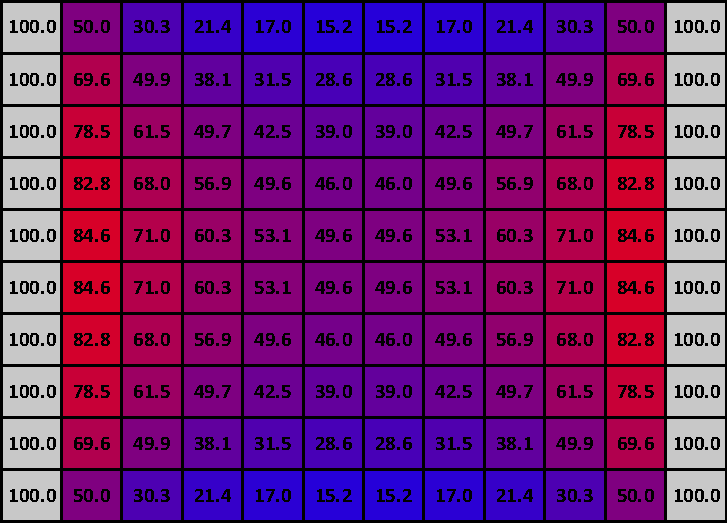
\includegraphics[width=0.6\textwidth]{papers/parallelisierung/images/simulation_10x10_0.135.pdf}
	\caption{Temperaturverteilung für \(10\times 10\)-Gitter, \(\lambda = 0.135\), nach Konvergenz.}
	\label{parallelisierung:fig:simulation-10x10-0-135}
\end{figure}

\paragraph{Fall 2: Instabile Simulation}  
Erhöhen wir die Auflösung auf \(15\times 15\) Messpunkte (\(\Delta l = 0.006\,\mathrm{m}\)), bei gleichem \(\Delta t = 1\,\mathrm{s}\), daraus folgt
\[
\lambda =
10^{-5} \cdot \frac{1}{0.006^2}
\approx 0.376 > \frac14.
\]
Diese Parameter verletzen die aus \eqref{parallelisierung:eq:stabForExp} hervorgehende Stabilitätsbedingung. Somit ist nun mit einer Simulation zu rechnen die nicht wie zuvor sauber konvergiert sondern mit dem fortschreiten der Zeit immer instabiler wird.

\begin{figure}[htbp]
	\centering
	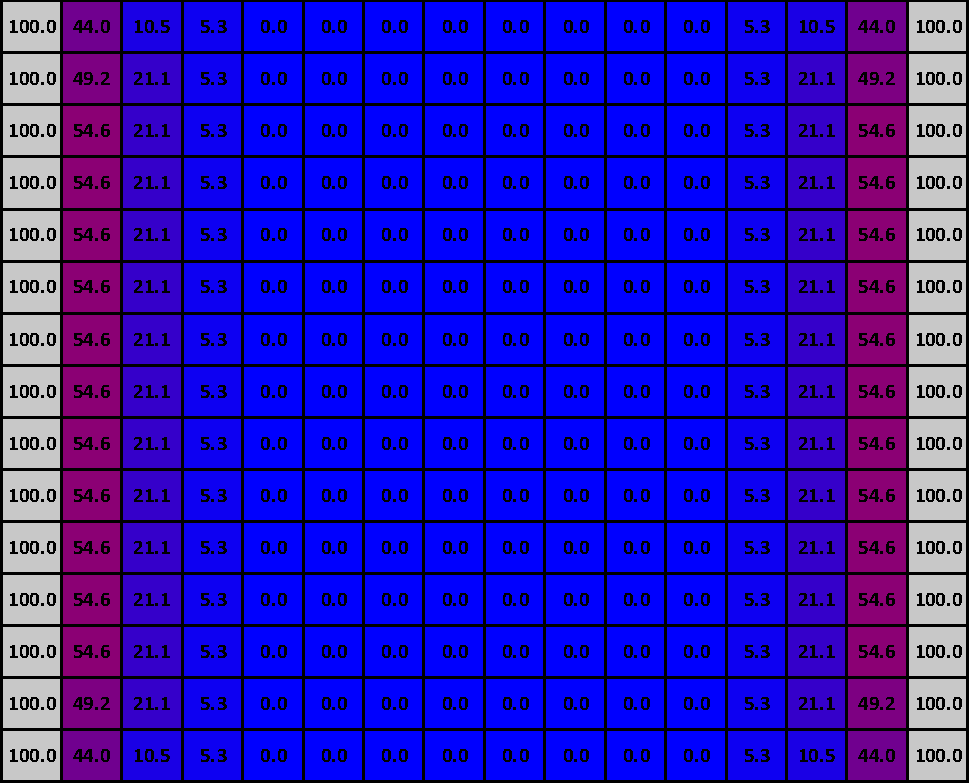
\includegraphics[width=0.6\textwidth]{papers/parallelisierung/images/simulation_15x15_0.376_3it.pdf}
	\caption{\(15\times 15\)-Gitter, \(\lambda = 0.376\), nach 3 Iterationen.}
	\label{parallelisierung:fig:simulation-15x15-0-376-3it}
\end{figure}

\begin{figure}[htbp]
	\centering
	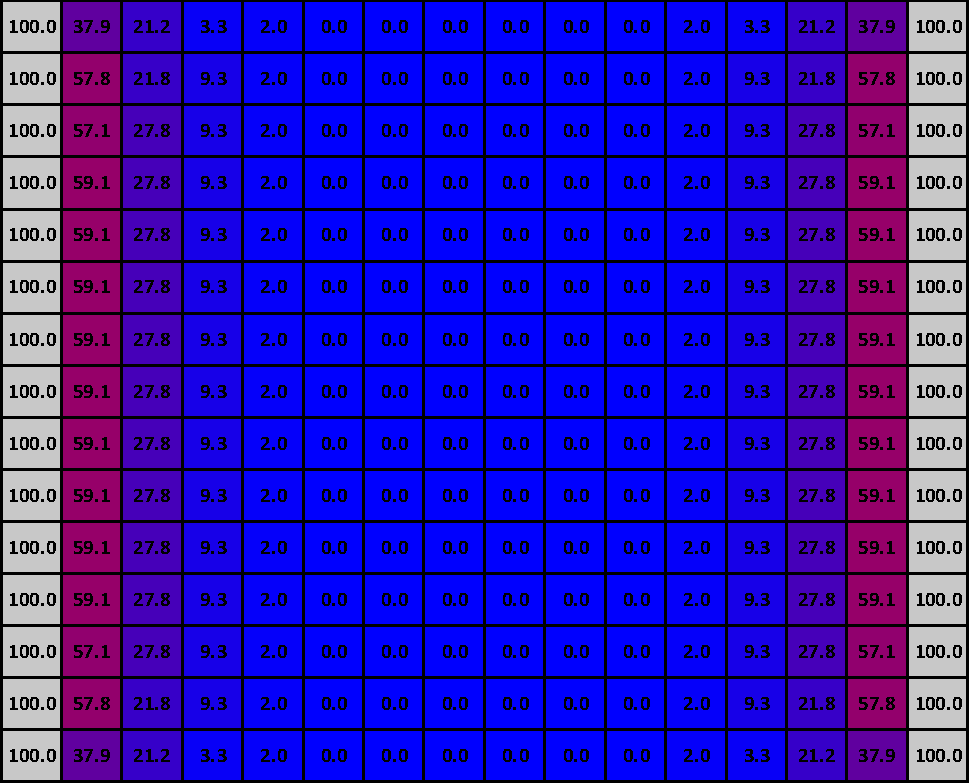
\includegraphics[width=0.6\textwidth]{papers/parallelisierung/images/simulation_15x15_0.376_4it.pdf}
	\caption{\(15\times 15\)-Gitter, \(\lambda = 0.376\), nach 4 Iterationen: erste Instabilitätsartefakte.}
	\label{parallelisierung:fig:simulation-15x15-0-376-4it}
\end{figure}

Zunächst scheint die Simulation noch plausibel (Abbildung~\ref{parallelisierung:fig:simulation-15x15-0-376-3it}), doch bereits nach wenigen Iterationen erscheinen die ersten auffälligen Werte (orange Zahlen in Abbildung~\ref{parallelisierung:fig:simulation-15x15-0-376-4it}). Anhand der physikalischen Intuition sowie den Ergebnissen der stabilen Simulation ist bekannt, dass das Temperaturgefälle von jeder Zelle in der oberen bzw. unteren Hälfte der Metallplatte bei jedem weiteren Schritt nach oben respektive unten entlang der orangen Pfeile streng monoton fallend sein muss. Das heißt, es kann nicht plötzlich wieder heißer werden, obwohl wir näher an den Rand gehen. Daraus lässt sich schließen, dass die orange markierten Werte unphysikalisch und somit erste Instabilitäts-Artefakte sind.


Die Ursache lässt sich durch Umformung der Update-Formel verdeutlichen mit
\begin{equation}
	T_{i,j}^{n+1}
	=
	(1-4\lambda)T_{i,j}^n +
	\lambda \left(
	T_{i+1,j}^n + T_{i-1,j}^n + T_{i,j+1}^n + T_{i,j-1}^n
	\right).
\end{equation}
Für \(\lambda > \tfrac14\) wird der Koeffizient \((1-4\lambda)\) negativ was widerum bedeutet das das Zentrum negativ gewichtet wird.  
Dies führt dazu, dass Unterschiede zwischen benachbarten Zellen nicht geglättet, sondern verstärkt werden: es entstehen Über- und Unterschwinger, die sich mit jeder Iteration vergrößern.

\begin{figure}[htbp]
	\centering
	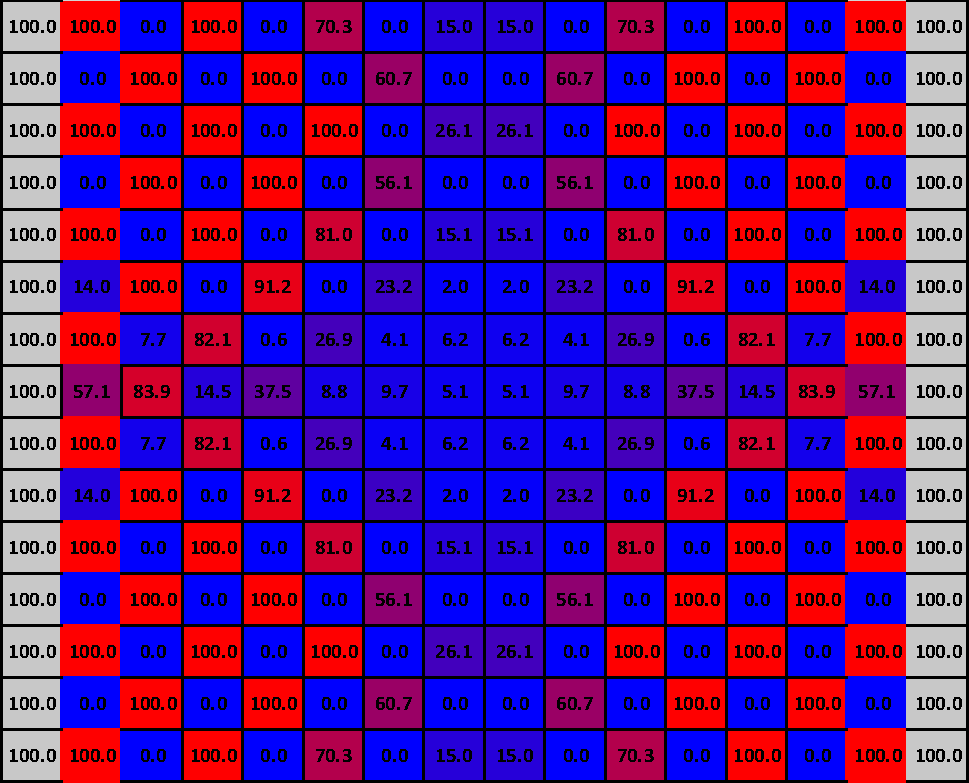
\includegraphics[width=0.6\textwidth]{papers/parallelisierung/images/simulation_15x15_0.376_15it.pdf}
	\caption{\(15\times 15\)-Gitter, \(\lambda = 0.376\), nach 15 Iterationen: klare Instabilitätsartefakte.}
	\label{parallelisierung:fig:simulation-15x15-0-376-15it}
\end{figure}

Lediglich 10 Iterationen später zeigt sich das Verhalten gemäss Abbildung~\ref{parallelisierung:fig:simulation-15x15-0-376-15it}, hier ist die Instabilität der Simulation aufgrund der Verletzung der 2D Stabilitätbedinung mit \(\lambda = 0.376 > \frac{1}{4}\) deutlich Sichtbar.

\paragraph{Fall 3: Wiederherstellung der Stabilität}  
Durch Verringerung von \(\Delta t\) auf \(0.5\,\mathrm{s}\) ergibt sich
\[
\lambda =
\frac{50}{7850 \cdot 470} \cdot \frac{0.5}{0.006^2}
\approx 0.188 < \frac14,
\]
wodurch die Simulation wieder stabil wird. Die Konvergenz wird nach 315 Iterationen erreicht (Abbildung~\ref{parallelisierung:fig:simulation-15x15-0-188-konv}).

\begin{figure}[htbp]
	\centering
	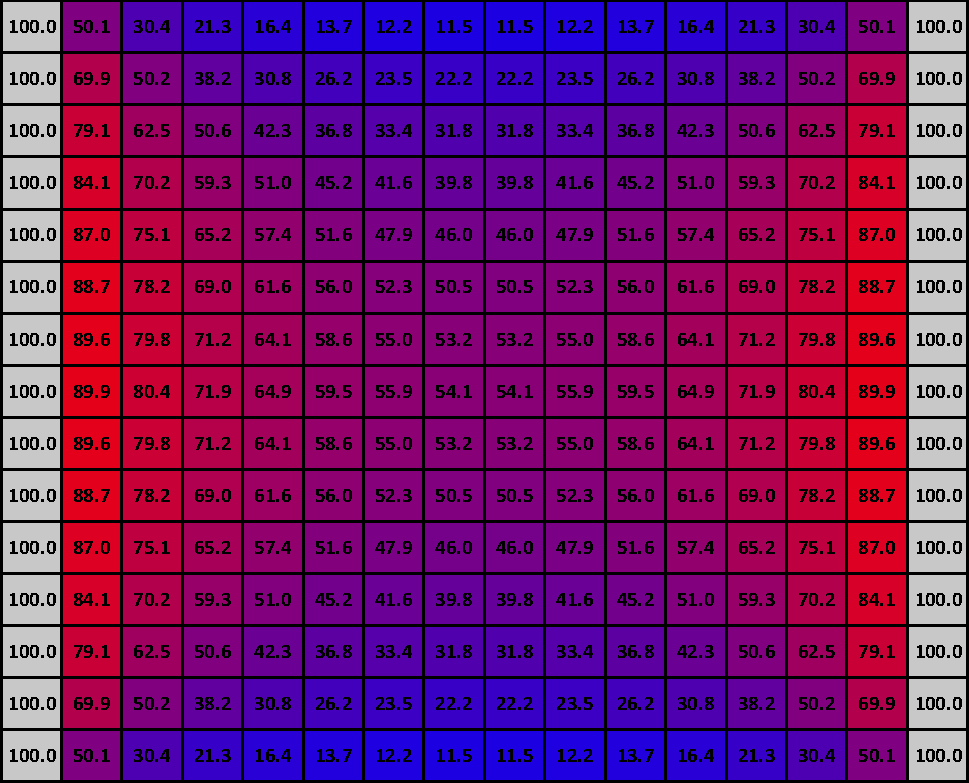
\includegraphics[width=0.6\textwidth]{papers/parallelisierung/images/simulation_15x15_0.188_konv.pdf}
	\caption{\(15\times 15\)-Gitter, \(\lambda = 0.188\), stabil nach Konvergenz.}
	\label{parallelisierung:fig:simulation-15x15-0-188-konv}
\end{figure}



%Hast du gut gemacht
% einleitung.tex -- Beispiel-File für die Einleitung
%
% (c) 2020 Prof Dr Andreas Müller, Hochschule Rapperswil
%
% !TEX root = ../../buch.tex
% !TEX encoding = UTF-8
\section{Gebietsunterteilung}
\label{parallelisierung:sec:Gebietsunterteilung}
\kopfrechts{Gebietsunterteilung}


\subsection{Motivation}
Wie aus dem Abschnitt der numerischen Methoden hervorgeht, führt eine Verfeinerung der Raum- und Zeitauflösung zwar zu genaueren Ergebnissen, jedoch auch zu mehr Datenpunkten und somit einem erheblich höheren Rechenaufwand. 
Mit zunehmender Gitterfeinheit steigt die Anzahl der Unbekannten quadratisch (in 2D) bzw. kubisch (in 3D).  
Um diese steigende Komplexität effizient bewältigen zu können, bietet sich die Gebietsunterteilung an.

Feldgleichungen wie die Wärmeleitungsgleichung besitzen wie im ersten Abschnitt dieser Arbeit erklärt eine lokale Struktur.
Also hängt der Wert in einem Gitterpunkt nur von seinen direkten Nachbarn (räumlich und zeitlich) ab.  
Diese Eigenschaft erlaubt es, ein grosses Problem in kleinere Teilprobleme zu zerlegen, sie getrennt zu berechnen und anschliessend wieder zusammenzufügen.

\subsection{Mathematische Zerlegung}
Sei $\Omega \subset {R}^2$ das Gesamtgebiet, diskretisiert durch ein kartesisches Gitter.  
Nun zerlegen wir $\Omega$ in $P$ disjunkte Teilgebiete $\Omega_p$:
\begin{equation}
	\Omega = \bigcup_{p=1}^P \Omega_p,
	\qquad 
	\Omega_p \cap \Omega_q = \emptyset \quad \text{für } p \neq q.
\end{equation}

Das bedeutet:
\begin{itemize}
	\item Das Gesamtgebiet setzt sich vollständig aus den Teilgebieten zusammen.
	\item Jedes Gitterelement gehört genau zu einem Teilgebiet.
	\item Die Teilgebiete überlappen sich nicht, können sich aber an den Rändern berühren.
\end{itemize}

Anschaulich entspricht dies einem Puzzle: 
jedes Teilgebiet ist ein Puzzlestück, das nahtlos mit den Nachbarstücken zusammenpassen muss.

\subsection{Kopplungsbedingungen}
Damit die Zerlegung konsistent bleibt, müssen an den Schnittstellen (Rändern) bestimmte Bedingungen erfüllt sein:

\paragraph{Stetigkeit der Lösung.}
\index{Stetigkeit der Lösung}%
\begin{equation}
	T_{\Omega_p}(x,y,t) = T_{\Omega_q}(x,y,t)
	\qquad \forall (x,y) \in \partial \Omega_p \cap \partial \Omega_q.
\end{equation}
Die Temperatur darf an den Schnittkanten keine Sprünge zeigen.

\paragraph{Stetigkeit des Flusses.}
\index{Stetigkeit des Flusses}%
\begin{equation}
	- \kappa \, \nabla T_{\Omega_p} \cdot n
	=
	- \kappa \, \nabla T_{\Omega_q} \cdot n
	\qquad \forall (x,y) \in \partial \Omega_p \cap \partial \Omega_q.
\end{equation}
Es darf keine künstliche Wärmequelle oder -senke entstehen: der aus einem Gebiet austretende Fluss tritt ins Nachbargebiet ein.

\subsection{Diskrete Umsetzung mit Ghost-Zellen}
Betrachten wir erneut die zweidimensionale Wärmeleitungsgleichung
\begin{equation}
	\frac{\partial T}{\partial t} = 
	\alpha \left(
	\frac{\partial^2 T}{\partial x^2} + \frac{\partial^2 T}{\partial y^2}
	\right).
\end{equation}
Zur Wiederholung: Mit FDM ergibt sich für ein quadratisches Gitter mit $\Delta l=\Delta x=\Delta y$ die Update-Formel
\begin{equation}
	T_{i,j}^{n+1}
	=
	T_{i,j}^{n}
	+
	\lambda \left(
	T_{i+1,j}^{n}+T_{i-1,j}^{n}+T_{i,j+1}^{n}+T_{i,j-1}^{n}-4\,T_{i,j}^{n}
	\right),
	\quad
	\lambda=\frac{\alpha\Delta t}{(\Delta l)^2}.
	\label{eq:update-dd}
\end{equation}

Für innere Punkte eines Teilgebiets $\Omega_p$ kann \eqref{eq:update-dd} direkt berechnet werden.  
An Schnittkanten hingegen benötigt man Werte aus Nachbargebieten.  
Dazu führt man sogenannte Ghost-Zellen ein:
\begin{itemize}
	\item Sie enthalten Kopien der Randwerte aus benachbarten Teilgebieten.
	\item Nach jedem Zeitschritt werden sie synchronisiert.
\end{itemize}
So kann jedes Teilgebiet lokal weiterrechnen. Dies erlaubt eine effiziente Parallelisierung, da nur die Schnittkanten kommuniziert werden müssen.

Abbildung~\ref{parallelisierung:fig:ghostCells} zeigt exemplarisch, wie an den Rändern benachbarter Teilgebiete Daten ausgetauscht werden. Farblich orange hervorgehoben sind die Ghost-Zellen.

\begin{figure}
	\centering
	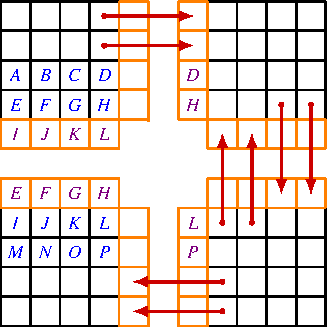
\includegraphics{papers/parallelisierung/images/ghostCells.pdf}
	\caption{Funktionsweise der Ghost-Zellen}
	\label{parallelisierung:fig:ghostCells}
\end{figure}



\subsection{Speziallfall: Stationärer Grenzfall}
Für $n \to \infty$ strebt das Zeitschrittverfahren gegen ein stationäres Temperaturfeld. 
Dann verschwindet die Zeitableitung, und die Wärmeleitungsgleichung reduziert sich auf die Laplace-Gleichung
\[
\nabla^2 T = 0.
\]

Diskretisiert mit FDM erhält man für jeden inneren Gitterpunkt eine lineare Beziehung zu seinen Nachbarn:
\[
-4T_{i,j} + T_{i+1,j} + T_{i-1,j} + T_{i,j+1} + T_{i,j-1} = 0.
\]

Alle diese Gleichungen zusammen bilden ein lineares System
\[
\mathbf{A}\vec{u} = \vec{b}.
\]

\subsubsection{Beispiel: $5\times 5$-Gitter}

Einmal mehr legen wir uns ein Beispiel zurecht um dies besser zu verstehen. Dieses mal nehmen wir  ein $5\times 5$-Gitter mit folgenden Randwerten:
\[
T=100^\circ\mathrm{C}\ \text{(links)},\quad
T=0^\circ\mathrm{C}\ \text{(rechts)},\quad
T=80^\circ\mathrm{C}\ \text{(oben)},\quad
T=20^\circ\mathrm{C}\ \text{(unten)}.
\]
\begin{figure}
	\centering
	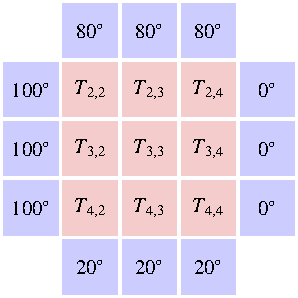
\includegraphics{papers/parallelisierung/images/stationaer.pdf}
	\caption{Beispiel-Setup $5\times5$-Grid für den stationären Grenzfall}
	\label{parallelisierung:fig:stationaer}
\end{figure}
Daraus ergeben sich $3\times 3 = 9$ innere Unbekannte.
Zusätzlich entfernen wir aus Gründen der Übersicht die Randzellen ohne Einfluss auf die inneren Zellen. Somit resultiert das Modell gemäss Abbildung \ref{parallelisierung:fig:stationaer}.


\subsubsection*{Diskretisierung}
Wenden wir nun die zuvor hergeleitete explizite Updateformel \eqref{eq:update-dd} auf dieses Gitter an, resultieren die folgenden 9 Gleichungen:
\begin{equation*}
\renewcommand{\arraycolsep}{3pt}
\begin{array}{cclclclclcl}
	-4\color{darkred}{T_{2,2}} &+& T_{3,2} &+& 80      &+& T_{2,3} &+& 100     &=& 0, \\
	-4\color{darkred}{T_{2,3}} &+& T_{3,3} &+& 80      &+& T_{2,4} &+& T_{2,2} &=& 0, \\
	-4\color{darkred}{T_{2,4}} &+& T_{3,4} &+& 80      &+& 0       &+& T_{2,3} &=& 0, \\
	-4\color{darkred}{T_{3,2}} &+& T_{4,2} &+& T_{2,2} &+& T_{3,3} &+& 100     &=& 0, \\
	-4\color{darkred}{T_{3,3}} &+& T_{4,3} &+& T_{2,3} &+& T_{3,4} &+& T_{3,2} &=& 0, \\
	-4\color{darkred}{T_{3,4}} &+& T_{4,4} &+& T_{2,4} &+& 0       &+& T_{3,3} &=& 0, \\
	-4\color{darkred}{T_{4,2}} &+& 20      &+& T_{3,2} &+& T_{4,3} &+& 100     &=& 0, \\
	-4\color{darkred}{T_{4,3}} &+& 20      &+& T_{3,3} &+& T_{4,4} &+& T_{4,2} &=& 0, \\
	-4\color{darkred}{T_{4,4}} &+& 20      &+& T_{3,4} &+& 0       &+& T_{4,3} &=& 0.
\end{array}
\end{equation*}

\subsubsection*{Matrixformulierung}
Wir ordnen die Unbekannten zeilenweise:
\[
\vec{u} =
\begin{pmatrix}
	T_{2,2}\\T_{2,3}\\T_{2,4}\\
	T_{3,2}\\T_{3,3}\\T_{3,4}\\
	T_{4,2}\\T_{4,3}\\T_{4,4}
\end{pmatrix}.
\]
Dann gilt:
\[
\mathbf{A}\vec{u}=\vec{b},
\]
mit
\[
\mathbf{A}=
\begin{pmatrix*}[r]
	-4& 1& 0& 1& 0& 0& 0& 0& 0\\
	1&-4& 1& 0& 1& 0& 0& 0& 0\\
	0& 1&-4& 0& 0& 1& 0& 0& 0\\
	1& 0& 0&-4& 1& 0& 1& 0& 0\\
	0& 1& 0& 1&-4& 1& 0& 1& 0\\
	0& 0& 1& 0& 1&-4& 0& 0& 1\\
	0& 0& 0& 1& 0& 0&-4& 1& 0\\
	0& 0& 0& 0& 1& 0& 1&-4& 1\\
	0& 0& 0& 0& 0& 1& 0& 1&-4
\end{pmatrix*},
\quad
\vec{b}=
\begin{pmatrix*}[r]
	-180\\-80\\-80\\
	-100\\0\\0\\
	-120\\-20\\-20
\end{pmatrix*}.
\]

\subsubsection*{Interpretation und Lösung}
\begin{itemize}
	\item $\mathbf{A}$ ist dünnbesetzt und spiegelt die 5-Punkt-Nachbarschaft wider.
	\item $\vec{b}$ enthält die Beiträge der Randwerte (verschieden je nach Position).
	\item Das System besitzt eine eindeutige Lösung: es liefert eine schräg verlaufende Temperaturverteilung zwischen den warmen und kalten Rändern.
\end{itemize}

\subsubsection*{Bemerkung zur Gebietsunterteilung im stationären Fall.}  
Im zeitabhängigen Fall werden Ghost-Zellen bei jedem Zeitschritt mit den Werten der Nachbargebiete gefüllt.  
Im stationären Fall dagegen gibt es keine Iteration in der Zeit, sodass die Ghost-Werte nicht direkt verfügbar sind.  
Um die Kopplung zwischen Subdomains herzustellen, gibt es zwei grundsätzliche Ansätze:

\begin{itemize}
	\item \emph{Algebraischer Ansatz:}  
	Das Gesamtsystem wird als grosse Blockmatrix aufgestellt.  
\index{Blockmatrix}%
	Jeder Hauptdiagonalblock \(A_{pp}\) beschreibt die inneren Zusammenhänge (die ``Selbstkopplung'') innerhalb eines Teilgebiets~\(\Omega_p\).  
\index{Hauptdiagonalblock}%
\index{Nebendiagonalblock}%
	Die Nebendiagonalblöcke \(C_{pq}\) modellieren die Kopplungen zu den Nachbargebieten~\(\Omega_q\).  
	
	Zur Illustration nehmen wir ein Beispiel mit drei Teilgebieten.  
	Das Gesamtsystem hat dann die Form
	\[
	\mathbf{A} =
	\begin{bmatrix}
		A_{11} & C_{12} & C_{13} \\
		C_{21} & A_{22} & C_{23} \\
		C_{31} & C_{32} & A_{33}
	\end{bmatrix}
	\]
	Hier enthält jeder Block \(A_{pp}\) die Koeffizienten für die inneren Punkte von~\(\Omega_p\), 
	während \(C_{pq}\) nur Einträge für die Schnittkanten trägt.  
	
	Durch Verfahren wie das Schur-Komplement kann die Lösung des Gesamtsystems auf die Werte an den Interfaces reduziert werden, 
\index{Schur-Komplement}%
	wodurch die Rechenlast deutlich sinkt.  
	Weiterführende Details finden sich beispielsweise in \cite{parallelisierung:smith1996}.
	
	\item \emph{Iterative Ansätze:}  
	Domain-Decomposition-Verfahren berechnen die Teilgebiete wiederholt und tauschen dabei nach jeder Iteration die Werte an den Schnittkanten aus, bis Konsistenz erreicht ist.  
	
	Ein klassisches Beispiel ist die \emph{Schwarz-Methode}.  
\index{Schwarz-Methode}%
	Hier werden an den künstlichen Rändern zwischen den Teilgebieten \emph{Dirichlet-Randbedingungen} vorgegeben, d.\,h.\ die benachbarten Teilgebiete liefern feste Temperaturwerte, die als Randwerte eingesetzt werden.  
\index{Dirichlet-Randbedingungen}%
	Genau diese Art von Randbedingungen haben wir auch im obigen Beispiel mit festen Temperaturen an den Aussenrändern des Gitters verwendet.  
	Die Schwarz-Methode ist einfach und robust, kann jedoch bei vielen Teilgebieten langsam konvergieren.  
	Eine ausführliche Darstellung findet sich in \cite{parallelisierung:quarteroniValli1999}.  
	
	Eine leistungsfähigere Alternative ist die \emph{Neumann--Neumann-Methode}.  
	In diesem Verfahren werden an den Schnittkanten \emph{Neumann-Randbedingungen} eingesetzt, also Bedingungen für die Flüsse (z.\,B.\ Wärmeströme) über die Gebietsgrenzen hinweg.  
\index{Neumann-Randbedingungen}%
	Die Subdomänen werden parallel berechnet, und die Flusswerte an den Interfaces werden iterativ korrigiert, bis Konsistenz erreicht ist.  
	Dieser Ansatz eignet sich besonders für elliptische Probleme und skaliert gut auf parallelen Rechnerarchitekturen.  
	Details hierzu finden sich in \cite{parallelisierung:gander2019}.
\end{itemize}


\subsection{Praktische Aspekte}

\subsubsection {Lastverteilung und Kommunikation}
Die Kosten pro Zeitschritt sind proportional zur Anzahl der Gitterpunkte im Teilgebiet 
($\mathcal{O}(|\Omega_p|)$).  
Die Kommunikationskosten entstehen durch den Austausch von Ghost-Zellen und hängen von der Länge der Schnittkante ab.  
\index{Kommunikationskosten}%
Für eine effiziente Parallelisierung ist es daher vorteilhaft, Teilgebiete mit möglichst kleinem 
Umfang/Flächen-Verhältnis zu wählen.  
In 2D bedeutet dies, dass quadratische Teilgebiete günstiger sind als lange, schmale Streifen.
Im 3D-Fall spricht man analog vom Oberflächen/Volumen-Verhältnis.  

\subsubsection {Stabilität}
Die Stabilitätskriterien der expliziten Finite-Differenzen-Methode gelten auch bei der Gebietsunterteilung unverändert.  
Insbesondere muss in 2D für ein quadratisches Gitter stets
\[
\lambda = \frac{\alpha \Delta t}{(\Delta l)^2} \leq \tfrac{1}{4}
\]
gelten.  
Diese Bedingung ist lokal in jedem Teilgebiet genauso einzuhalten wie global. 


%
% teil2.tex -- Beispiel-File für teil2 
%
% (c) 2020 Prof Dr Andreas Müller, Hochschule Rapperswil
%
% !TEX root = ../../buch.tex
% !TEX encoding = UTF-8
%
\section{Parallelisierung
\label{parallelisierung:sec:Parallelisierung}}
\kopfrechts{Parallelisierung}
Wir kennen nun numerische Verfahren, welche es einer Maschine erlaubt unsere Feldgleichungen zu berechnen.
Wir wissen auch, wie wir unser Feld in Teilgebiete unterteilen können.
Das gibt uns alle Werkzeuge, welche wir benötigen um die Berechnungen unserer Gleichungen auf mehrere Maschinen aufzuteilen.

Bei der Parallelisierung von Feldgleichungen in einem Multiprozessorsystem wird jedem Prozessor eines oder mehrere zusammenhängende Teilgebiete zugewiesen.
Die Teilgebiete müssen theoretisch nicht zusammenhängend sein aber um die Kommunikation zwischen Prozessoren zu minimieren ist dieses Vorgehen sinnvoll und üblich.
Da die Randzellen jedes Teilgebietes abhängig von den angrenzenden Zellen sind, siehe \ref{parallelisierung:sec:Gebietsunterteilung}, müssen die vorhandenen Informationen dieser Zellen zwischen Gebieten auf unterschiedlichen Prozessoren ausgetauscht werden.
Dieser Austausch ist mit erheblichem zeitlichen Aufwand verbunden.
Die Frage, wie fein ein Gitter in verschiedene Teilgebiete aufgeteilt werden soll, ist also immer eine optimierungs-Frage.
Man muss ein Optimum finden, wo der zeitliche Gewinn der parallelen Berechnung die zeitlichen Verluste der Interprozess-Kommunikation überwiegen.

%
% einleitung.tex -- Beispiel-File für die Einleitung
%
% (c) 2020 Prof Dr Andreas Müller, Hochschule Rapperswil
%
% !TEX root = ../../buch.tex
% !TEX encoding = UTF-8
%
\subsection{Kommunikation zwischen Gebieten
\label{parallelisierung:sub:Interprozess}}
Zuerst eine kurze Rekapitulation zu einigen Begrifflichkeiten, welche wichtig sind für die Welt der parallelen Programmierung.
Ein Prozessor ist eine physische Recheneinheit wie zum Beispiel eine CPU oder GPU.
Prozessoren sind meist aus mehreren Kernen aufgebaut.
Jeder Kern ist eine eigenständige Recheneinheit und hat privaten wie auch mit anderen Kernen geteilten Speicher.
Ein Prozess ist ein eigenständiges Programm, welches vom Betriebssystem alle nötigen Resourcen wie Speicher, Rechenzeit und Daten zugeteilt bekommt.
Threads sind Teilaufgaben eines Prozesses, die gleichzeitig auf den verschiedenen Kernen des Prozessors arbeiten und sich die Daten und den Speicher dieses Prozesses teilen.

Für das Austauschen von Daten zwischen Teilgebieten gibt es zwei häufig verwendete Parallele Programmier- und Kommunikationsschnittstellen, OpenMP und MPI.
Im folgen werden beide kurz vorgestellt.

\subsubsection{OpenMP}
OpenMP ist eine API, welche sehr einfach das erzeugen von Threads und die Kommunikation zwischen diesen ermöglicht.
Jedes Teilgebiet wird hier einem Thread zugeteilt. 
Da sich diese Threads den Speicher des Prozesses teilen, nutzt OpenMP Shared-Memory für den Austausch von Daten.
Bei OpenMP gibt es keinen Thread-eigenen Speicher.
Jeder Thread kann also auf die Randzellen anderer Threads zugreifen.
Dadurch benötigt es keine Kommunikation zwischen den Teilgebieten im engeren Sinn.

Für kleine Systeme ist OpenMP eine einfache und gute Lösung.
Da es aber auf Shared-Memory basiert ist es schlecht skalierbar.
Werden für grosse Berechnungen mehrere Prozessoren verwendet ist Shared-Memory oft nicht verfügbar.
Grosse Berechnungen möchte man oft auch auf verschiedene Maschinen aufteilen, was mit OpenMP nicht möglich ist.
Der einfache Aufbau für den Programmierer bedeutet außerdem weniger Kontrolle über die Datenverteilung.

\subsubsection{MPI}
MPI ist ein Message Passing Interface.
Es dient nicht dazu Prozesse oder threads zu erzeugen.
Diese Aufgabe muss vom Betriebssystem ausgeführt werden.

MPI stellt Funktionen zur Verfügung für eine effiziente Kommunikation mittels Nachrichten zwischen den Prozessen.
Diese Prozesse haben nicht zwingend einen Shared Memory bereich.
Es wird daher als Distributed-Memory-Programmiermodell bezeichnet.
Jedes Teilgebiet wird hier einem Prozess zugeteilt.
Die Informationen über angrenzende Teilgebiete wird mittels Nachrichten oder auch Messages zwischen den Prozessen ausgetauscht.
Der Programmierer muss explizit Datenverteilung und Kommunikation steuern, was zwar einiges mehr Programmieraufwand aber auch bessere Kontrolle über die Daten bedeutet.

MPI zeichnet sich besonders über eine gute Skalierbarkeit aus.
Da kein Shared Memory nötig ist, kann man über beliebig viele Knoten, zum Beispiel mehrere CPUs oder ganze Rechner, die Daten durch Messages austauschen.

Man kann MPI auch für Systeme mit Shared Memory als eine Art Universallösung verwenden.
In diesem Fall wird allerdings trotz einem geteiltem Speicherbereich erheblicher Overhead für Kommunikation produziert, welcher mit OpenMP vermieden werden könnte.
%
% einleitung.tex -- Beispiel-File für die Einleitung
%
% (c) 2020 Prof Dr Andreas Müller, Hochschule Rapperswil
%
% !TEX root = ../../buch.tex
% !TEX encoding = UTF-8
%
\subsection{Prozess Synchronisation \label{parallelisierung:subsection:Synchronisation}}
Lorem ipsum dolor sit amet, consetetur sadipscing elitr, sed diam
nonumy eirmod tempor invidunt ut labore et dolore magna aliquyam
erat, sed diam voluptua \cite{parallelisierung:bibtex}.
At vero eos et accusam et justo duo dolores et ea rebum.
Stet clita kasd gubergren, no sea takimata sanctus est Lorem ipsum
dolor sit amet.

Lorem ipsum dolor sit amet, consetetur sadipscing elitr, sed diam
nonumy eirmod tempor invidunt ut labore et dolore magna aliquyam
erat, sed diam voluptua.
At vero eos et accusam et justo duo dolores et ea rebum.  Stet clita
kasd gubergren, no sea takimata sanctus est Lorem ipsum dolor sit
amet.




\subsection{Beispiel an der allgemeinen Wärmeleitungsgleichung
\label{parallelisierung:sub:BeispielParallelisierung}}
Zum besseren Verständnis wollen wir mit OpenMP ein Konkretes Beispiel für die Parallelisierung der allgemeinen Wärmeleitungsgleichung realisieren.
Zum Vergleich wird auch die Serielle Vorgehensweise präsentiert.
Als Ausgangslage soll für ein Gitter von AxB Zellen C Updates durchgeführt werden.
Für jedes Update wird die Formel \ref{parallelisierung:eq:update_formel} aus Abschnitt \ref{parallelisierung:sec:update_formel} verwendet.
Links und Rechts der Zellen gibt es Reihen mit unveränderlicher Temperatur, welche einen Heiz- respektive Kühlkörper darstellen.
Ober- und unterhalb der Zellen gibt es Zeilen mit unveränderlicher Temperatur, welche die Umgebungstemperatur darstellen.
Diese Konstanten, wie auch $\lambda$ als Konstante für die Updateformel können alle im Main-File des Programms definiert werden und sind unveränderlich.

Beide Lösungen verwenden Arrays zur Zwischenspeicherung der Zellen.
Für Arrays werden gerne Vektoren aus der C++ Standar Library (STL) verwendet.
Für ein zweidimensionales Array wird zum Beispiel
\begin{lstlisting}
	std::vector<std::vector<double>> grid;
\end{lstlisting}
benützt.
Man muss sich allerdings bewusst sein, dass diese Variante keinen kontinuierlichen Bereich im Speicher reserviert.
Diese Variante speichert zuerst ein äußeres Array (Zeilen), und jede Zeile allokiert separat ihren eigenen Speicher.
Das verschlechtert enorm die Cache-Lokalität des Programms und damit die Performanz.
Als elegantere Lösung verwendet man bei numerischen Verfahren für partielle Differentialgleichungen eindimensionale Arrays und rechnet die Indizes mittels inline-Funktion um.
\begin{lstlisting}
	std::vector<double> grid(nx * ny);
	
	inline double& at(int i, int j) {
		return grid[i * nx + j];  // Row-major
	}
\end{lstlisting}
Damit garantiert man eine kontinuierliche Speicherung der Daten.

\subsubsection{Serielle Lösung}
\label{parallelisierung:sub:serLoesung}}
Zur Vorbereitung werden Zwei Arrays der Grösse 
\begin{equation}
	A+2 * B+2 
\end{equation}
angelegt. 

\begin{lstlisting}
	std::vector<double> grid(A * B);
	std::vector<double> gridNew(A * B);
\end{lstlisting}
Die Addition von zwei ist notwendig, um die Umgebenden Temperaturen speichern zu können.
In beiden Arrays wird nun die Umgebungstemperatur in die erste und letzte Zeile geschrieben.
Die jeweilige Temperatur der Heiz-/Kühlkörper wird in die erste und letzte Spalte geschrieben.
Das erste Array wird für die aktuellen Temperaturen der Zellen verwendet.
Als Ausgangspunkt kann in dieses die Umgebungstemperatur eingetragen werden.
Mit einer Schlaufe kann nun für alle A*B Zellen der neue Wert mit der Updateformel berechnet und in die entsprechende Zelle im zweiten Array geschrieben werden.
\begin{lstlisting}[caption={Update-Schritt (seriell)},label={parallelisierung:code:updateSeriel}]
	for (int i = 1; i < B - 1; ++i) {     // ueberspringt erste und letzte Zeile
		const int row = i * A;
		for (int j = 1; j < A - 1; ++j) { // ueberspringt erste und letzte Spalte
			const int idx   = row + j;
			const int up    = idx - A;
			const int down  = idx + A;
			const int left  = idx - 1;
			const int right = idx + 1;
			
			nextTemp[idx] = currentTemp[idx]
			+ lambda * (src[up] + src[down] + src[left] + src[right]
			- 4.0 * src[idx]);
		}
	}
\end{lstlisting}
Im Beispiel ist src ein Pointer auf das Array mit den aktuellen Werten und dst ist ein Pointer auf das Array mit den neuen Werten.
Bei der Verwendung von Vektoren erhält man die Adresse des ersten Eintrags mit der Funktion .data().
\begin{lstlisting}
	double* src = grid.data();
	double* dst = gridNew.data();
\end{lstlisting}

Ist die For-Schleife durchgerechnet, kann man die beiden Array elegant austauschen, indem man die beiden Pointer tauscht.
\begin{lstlisting}
	std::swap(src, dst);
\end{lstlisting}
Auf diese weise müssen keine Daten Verschoben werden was viel Zeit einspart.
Dieses Verfahren nennt man passend einen Ping-Pong-Ansatz.

In einer Schlaufe die C mal durchlaufen wird, und den Updatecode sowie den Swap aufruft kann das Array C mal aktualisiert und damit das fortschreiten der Zeit simuliert werden.

\subsubsection{parallele Lösung 
\label{parallelisierung:sub:parLoesung}}
Die Vorgehensweise bei der parallelen Lösung ist sehr ähnlich.
Es werden zwei Arrays verwendet, welche im Shared-Memory des Prozesses liegen.
Jeder Thread kann auf das gesamte Array mit den aktuellen Werten zugreifen und kann daher auch die Randzellen problemlos berechnen.
Jedem Thread wird ein Teilgebiet des gesamten Arrays zugewiesen.
Der Thread berechnet darin jede Zelle mit den vorhandenen aktuellen Werten und schreibt das Ergebnis an der entsprechenden Stelle in das neue Array.
Da auf dem alten Array keine Schreibaktionen getätigt werden gibt es keine Möglichkeit für Race conditions.
Zur Synchronisation wird am ende der Updateschlaufe eine Barriere gesetzt, welche den Thread am weitermachen hindert, bis jeder andere Thread seine Arbeit verrichtet hat.
Wird diese Barriere überschritten, hat ein Thread die Aufgabe, die Pointer der Arrays auszutauschen.
Eine zweite Barriere sorgt dafür, dass die anderen Threads warten, bis dieser Pointer-Swap durchgeführt wurde.



\printbibliography[heading=subbibliography]
\end{refsection}
